\documentclass[]{article}
\usepackage[left=2.5cm,right=2.5cm,top=2.5cm,bottom=2cm]{geometry}
\usepackage{setspace}
\usepackage{graphicx}
\usepackage{listings}
\lstset{language=Python, basicstyle=\small\ttfamily}

\begin{document}

\title{Turing \"ahnliche Muster aus zellul\"aren Automaten}
\author{ Einf\"uhrung in die Visualisierung\\ 
	\\
	Johanna Jansen, Jette von Postel, Julien Stengel\\}
\date{}
\maketitle

\onehalfspacing

\begin{figure}[h]
	\frame{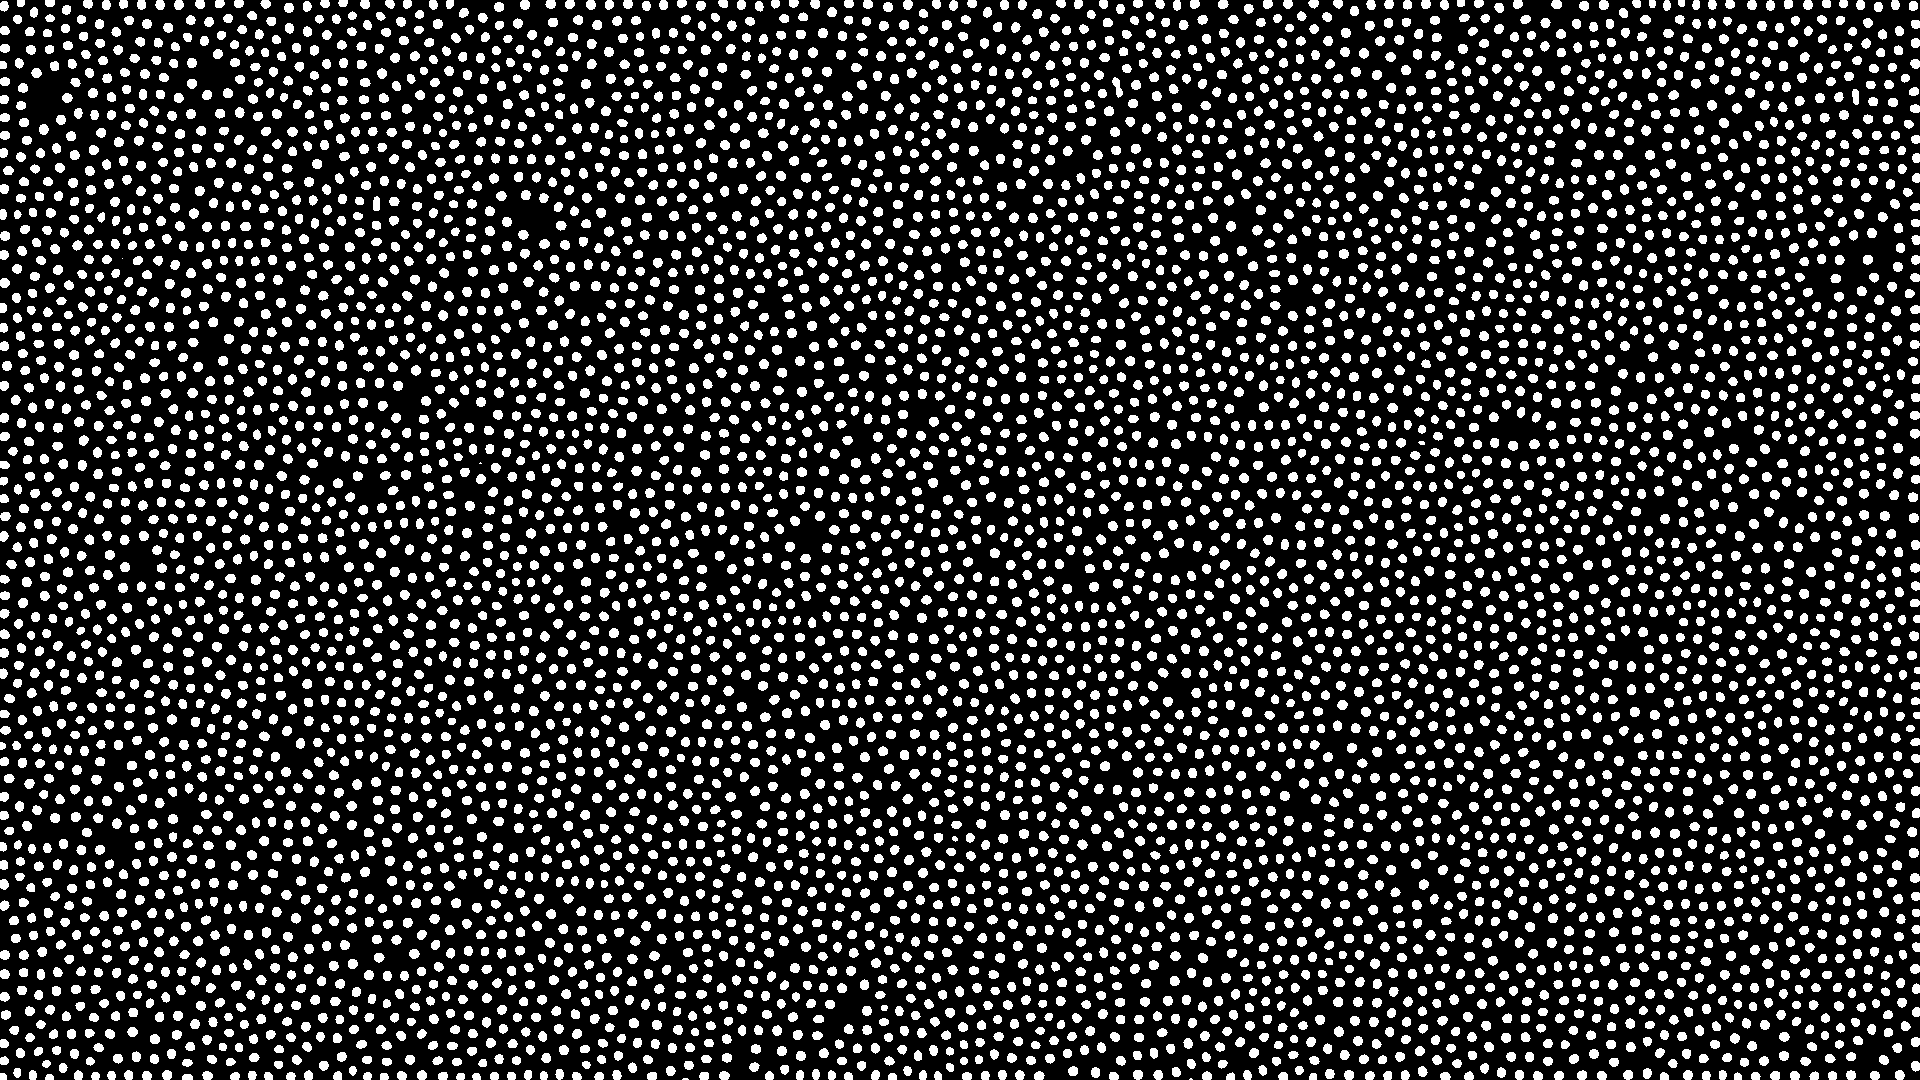
\includegraphics[trim=780 350 780 350, clip, width=0.22\textwidth]{punkte.png}}
	\hspace{10pt}
	\frame{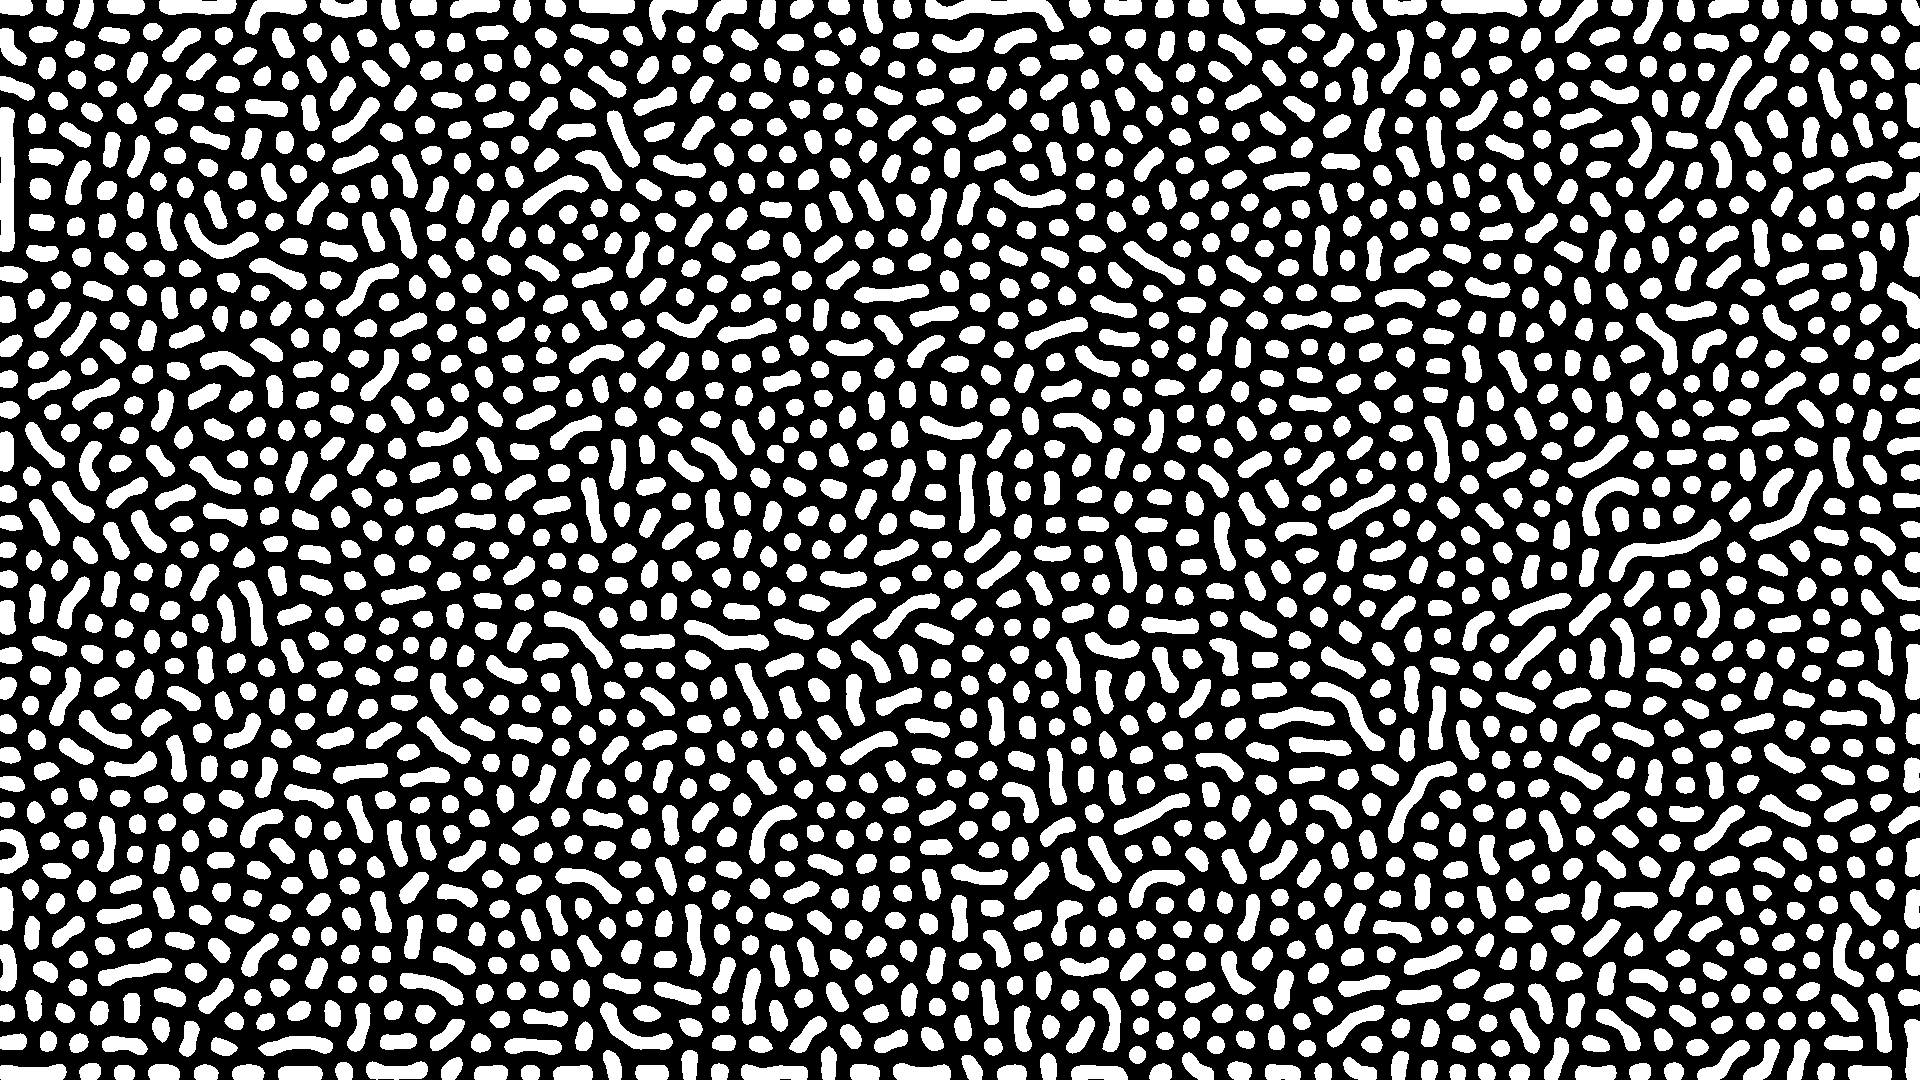
\includegraphics[trim=780 350 780 350, clip,width=0.22\textwidth]{halb.png}}
	\hspace{10pt}
	\frame{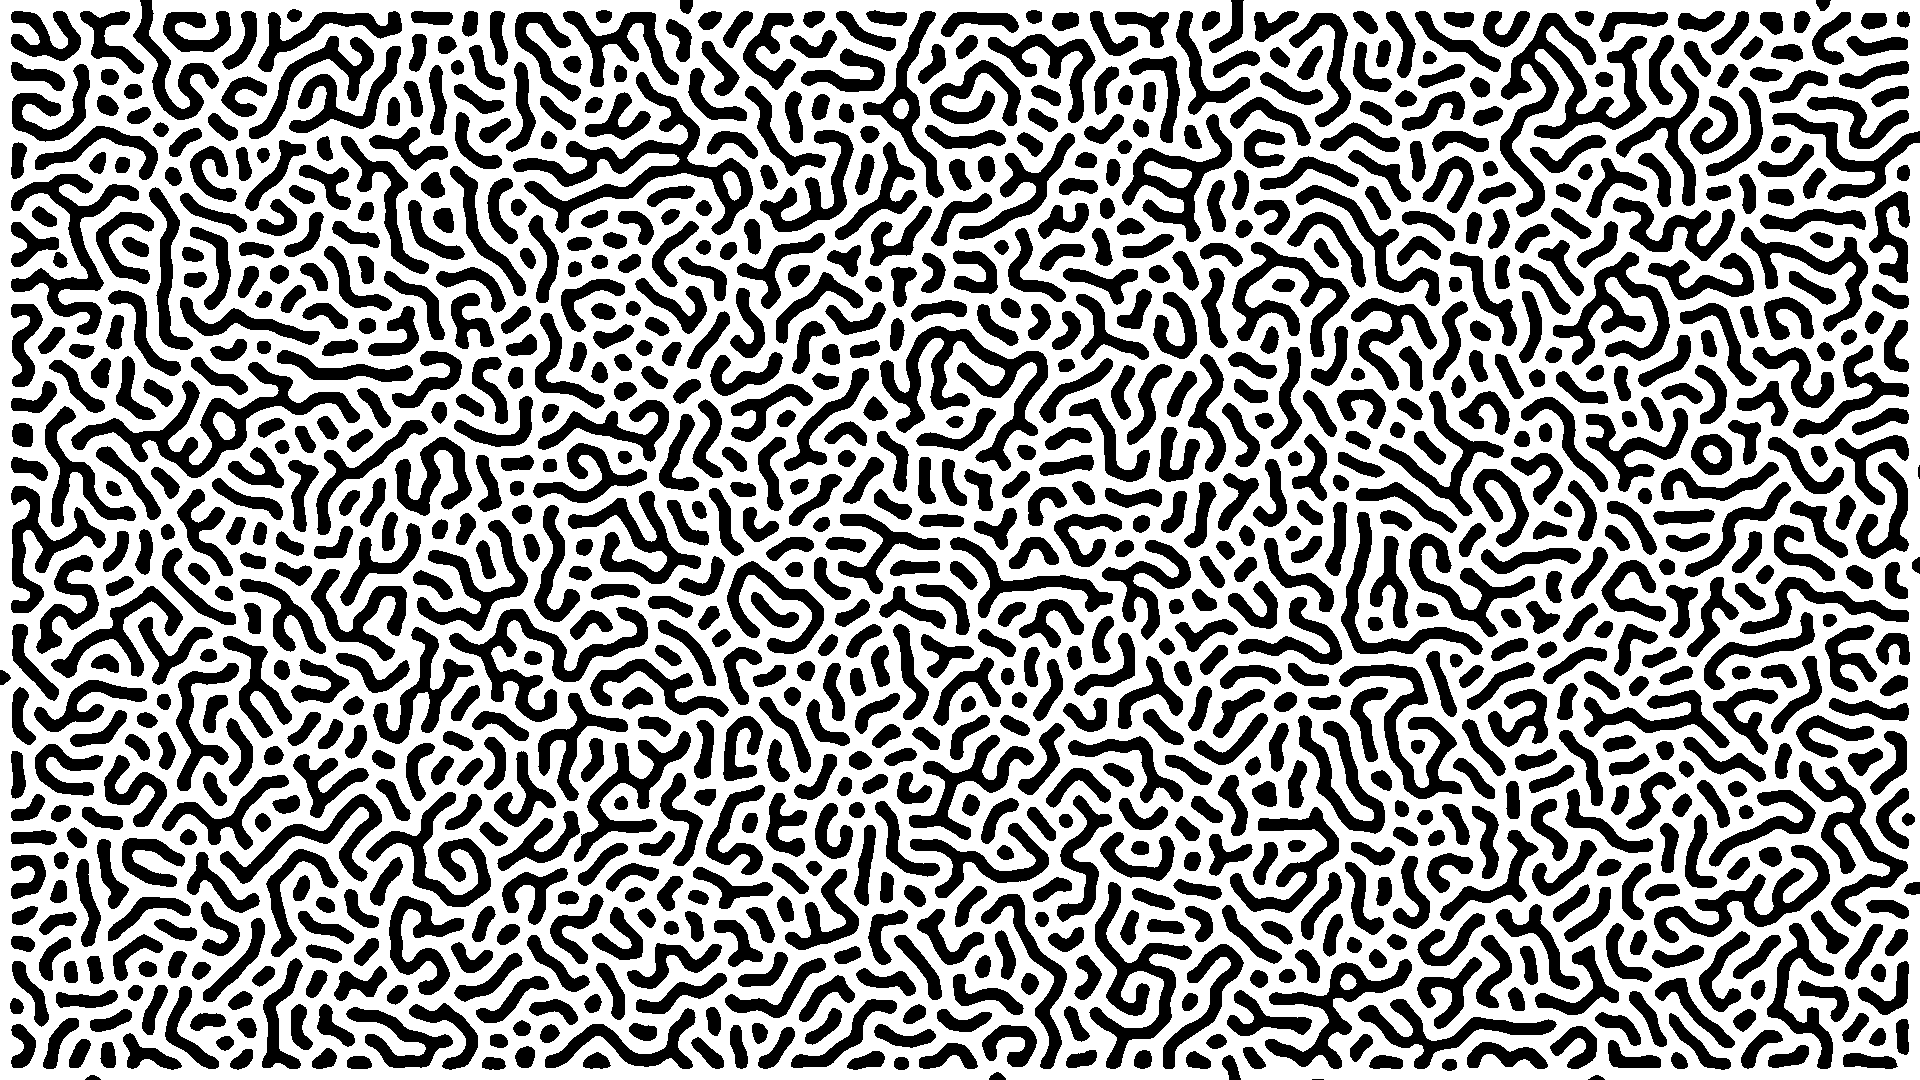
\includegraphics[trim=780 350 780 350, clip,width=0.22\textwidth]{labyrinth.png}}
	\hspace{10pt}
	\frame{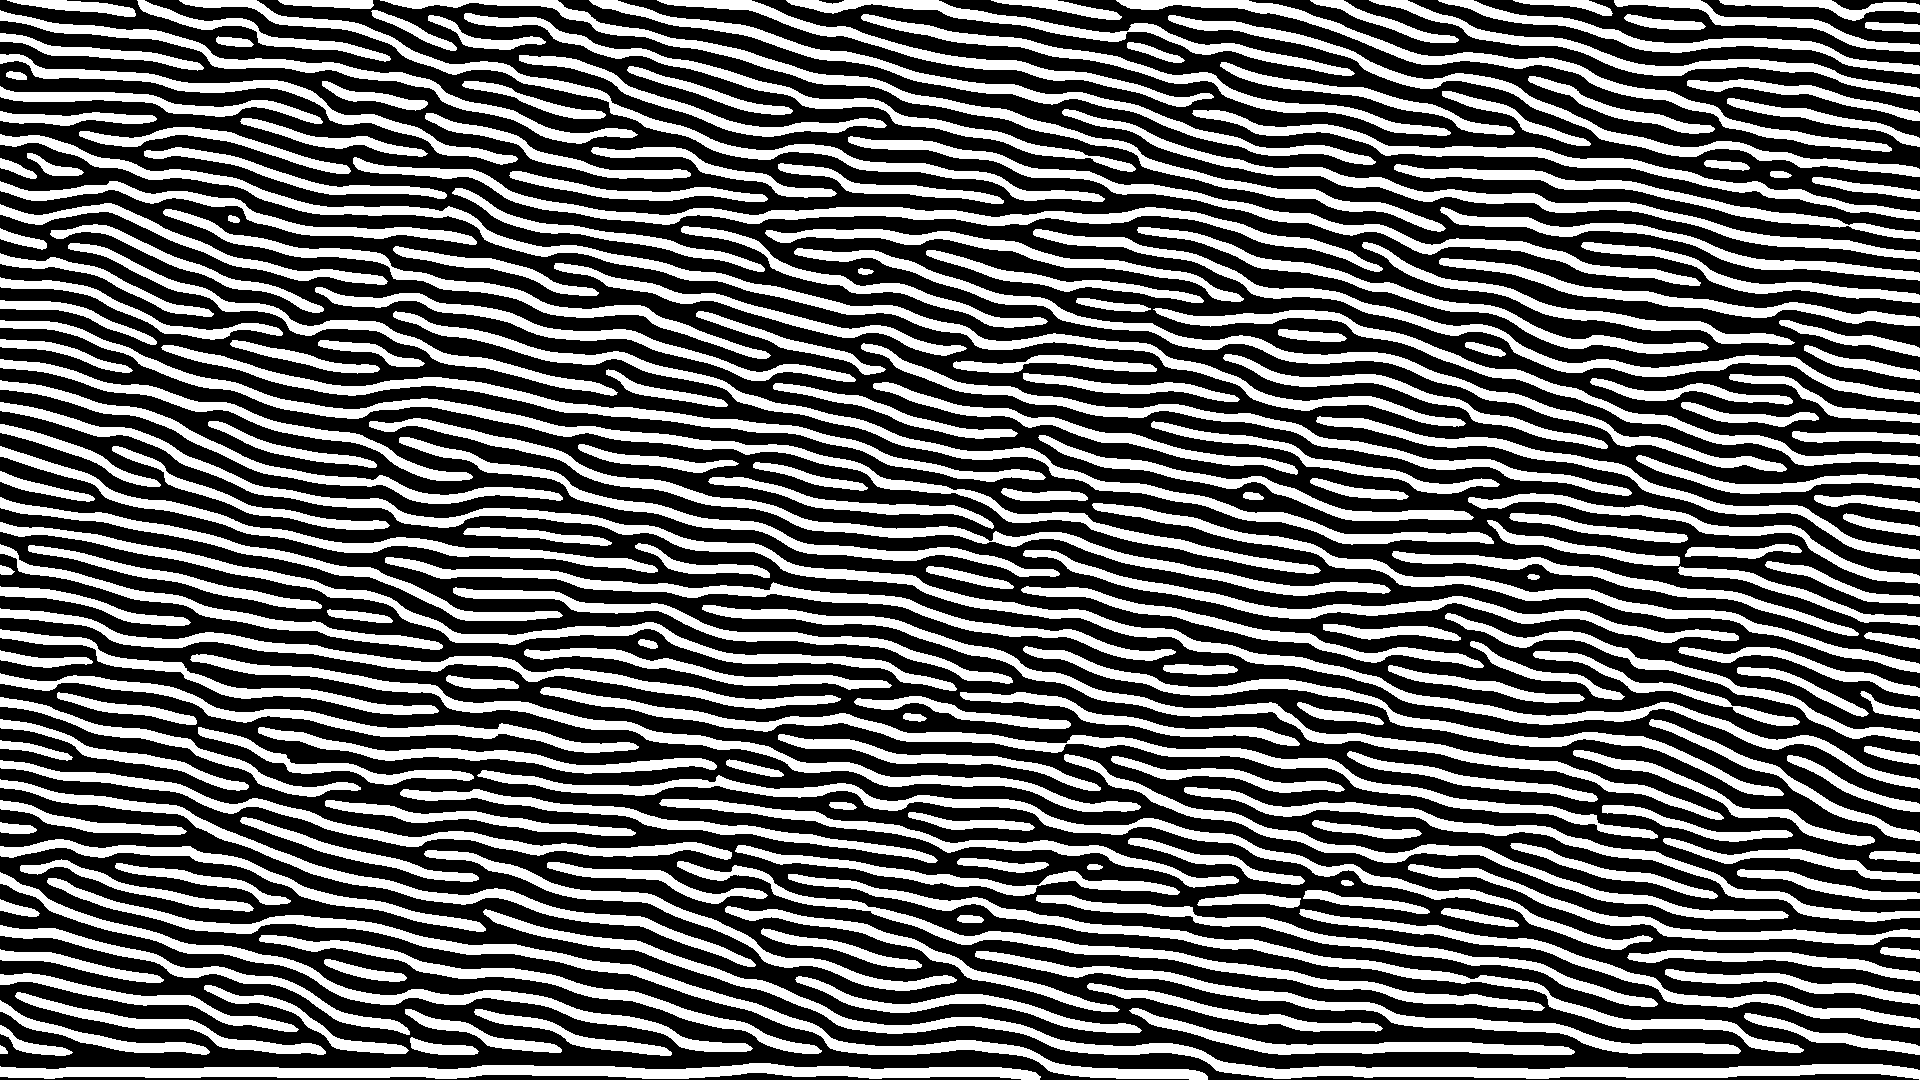
\includegraphics[trim=780 350 780 350, clip,width=0.22\textwidth]{zebra.png}}
\end{figure}

\section{Einleitung}

Auf der Bridges Finland Conference 2016 wurde eine Zusammenarbeit von Mathematikern und K\"unstlern zu Turing-\"ahnlichen Mustern vorgestellt. Im Rahmen des Seminars "Einf\"uhrung in die Visualisierung" haben wir diese Muster analysiert und reproduziert. 

\section{Das Turing Modell}

Der englische Mathematiker Alan Turing stellte 1952 einen Entwurf zur Modellierung stabiler r\"aumlicher Muster durch ein System aus Chemikalien oder Morphogenen vor, die bei unterschiedlich schneller Diffusion durch ein Substrat miteinander reagieren. Im Sinne einer biologischen Modellanwendung wirkt eines dabei kurzfristig aktivierend, w\"ahrend das andere eine langfristige hemmende Wirkung hat. \\

Das Modell ist gegeben durch die Anzahl der Zellen $C_i,~i=1,...,k$ und der  Morphogene $M_j, ~j=1,...,l$, sowie die Diffusionsraten der verschiedenen Morphogene. Jede Zelle $C_i$ enth\"alt nun Angaben zur Menge jedes Morphogens $M_j$ in dieser Zelle, $n_{C_i}(M_j)$. Diese Angaben \"andern sich durch Reaktion untereinander und Diffusion mit jedem Zeitschritt. Um diese \"Anderung feststellen zu k\"onnen, ist es genug, die Werte des gleichen Morphogens in den umliegenden Zellen $n_{C_i}(M_j), ~i=1,...,k$ zu kennen f\"ur eine Aussage zur Diffusion, sowie das Konzentrationsverh\"altnis aller Morphogene in der Zelle $n_{C_i}(M_j), ~j=1,...,l$ zur Betrachtung der chemischen Reaktionen. \\

Dieses an sich homogene System ist sehr anf\"allig f\"ur kleine Abweichungen, die es dann instabil machen und die Unregelm\"a\ss igkeiten wachsen l\"asst. Daraus entsteht ein neues stabiles System, was nicht mehr homogen ist, sondern verschiedene Muster aufweist. \\

Je mehr verschiedene Morphogene eine Zelle enth\"alt, desto komplizierter wird das Reaktions-Diffusions-System, das damit zusammenh\"angt.
F\"ur Systeme mit zwei Komponenten gibt es bereits viel mehr m\"ogliche Beobachtungen als im eindimensionalen Fall und Turings Idee, dass ein zun\"achst stabiler Zustand durch Diffusion instabil wird, wird wichtig.
Dies ist nur in einer bestimmten Klasse von Systemen m\"oglich, den \textit{activator-inhibitor systems}. Das bekannteste Beispiel daf\"ur ist die FitzHugh-Nagumo Gleichung 
	\begin{center}
	$\partial_t u = d^2_u \nabla^2 u + f(u) -\sigma v, $\\
	$\tau \partial_t v = d^2_v \nabla^2 v + u - v  $
	\end{center}
wobei $ f(u) = \lambda u - u^3 - \kappa $ beschreibt, wie Aktionspotential durch einen Nerv geleitet wird. Hier sind $ d_u, d_v, \tau, \sigma $ und $\lambda $ positive Konstanten.

Turing wollte mit diesem Morphogenese Modell eine biologische Erkl\"arung f\"ur Muster im Fell von Wirbeltieren finden.



\section{Das Young Modell}

Das erste Modell einer Implementierung von Turings Aktivierungs-Hemmungs-Konzept stammt von D.A. Young und ist ein diskreter zellul\"arer Automat. Er ist eine diskretisierte L\"osung einer verallgemeinerten Diffusionsgleichung. \\

Das Modell betrachtet eine Fl\"ache aus gleichgro\ss en Zellen, von denen einige gef\"arbt sind und einige nicht. Die Verteilung kann durch einen einfachen Zufallsprozess generiert werden. \\

Die gef\"arbten Zellen produzieren ein aktivierendes und ein hemmendes Gen. Das aktivierende Gen $M_1$ stimuliert umliegende ungef\"arbte Zellen gef\"arbt zu werden und das hemmende Gen $M_2$ hindert weiter entfernte gef\"arbte Zellen daran, gef\"arbt zu bleiben. 
Zusammen induzieren sie ein morphogenes Feld $w(R)$, wobei $R$ die Distanz zur gef\"arbten Zelle ist. Um die Zelle entsteht so ein innerer und ein \"au\ss erer Ring. Im inneren Ring hat $w(R)$ einen positiven Wert und im \"au\ss eren Ring einen negativen Wert. \\

In jedem Zeitschritt werden dann f\"ur jede Zelle mit Position \textbf{R} die Einfl\"usse ihrer Nachbarzellen mit Positionen \textbf{R$_i$} aufsummiert.

\begin{itemize}
	\item Wenn $\sum_{i} w (|$\textbf{R - R$_i$}$|)~>~0$, die Morphogen-Konzentration in der Zelle also positiv ist, dann wird bzw. bleibt die Zelle gef\"arbt. 
	
	\item Wenn $\sum_{i} w (|$\textbf{R - R$_i$}$|)~=~0$, dann bleibt die Zelle, wie sie ist. 
	
	\item Wenn $\sum_{i} w (|$\textbf{R-R$_i$}$|)~<~0$, die Morphogen-Konzentration in der Zelle also negativ ist, dann wird bzw. bleibt die Zelle ungef\"arbt. 
\end{itemize}

\section{Theoretische Umsetzung}
Zur Umsetzung in die Praxis stehen das urspr\"ungliche Turing-Modell und das Young-Modell zur Auswahl. 
Da jedoch das Young-Modell unter anderem zur einfachen Berechnung von Rechnern entwickelt wurde, haben wir uns f\"ur diese Methode der Generierung entschieden.
Man ben\"otigt also eine M\"oglichkeit ein Gitter darzustellen, in denen Zellen miteinander interagieren und sich dann aufgrund der Nachbarschaftsumgebung dynamisch anpassen k\"onnen.
Dabei werden Nachbarschaften als Kreis- oder Ellipsenringe betrachtet, sodass lebende Zellen im inneren Radius aktivierend und lebende Zellen im \"au\ss eren Radius eine hemmende Wirkung auf ihre Nachbarn haben. Verschiedene Formen dieser Nachbarschaftsringe produzieren dann verschiedene Muster als Ergebnisse.


\section{Praktische Umsetzung}

F\"ur die praktische Umsetzung haben wir uns f\"ur Python entschieden. Um genau zu sein, verwendeten wir den Spyder-Editor aus dem Anaconda-Paket, welcher uns im Kurs vorgestellt wurde. \\

Zur Berechnung der Muster entwickelten wir zwei Klassen, mit denen wir jeweils das Grid und die Zellen dargestellt und simuliert haben. 
Das Grid wird dar\"uber klassifiziert, dass es eine Zeilen- und Spaltenl\"ange hat. Zus\"atzlich wird es mit einer Chance versehen, mit der es am Anfang der Initialisierung eine Aktivatorzelle erstellt. Gibt man also als Startwerte f\"ur das Grid die folgenden Werte ein:
\begin{center}
	Zeilenl\"ange = 1980; Spaltenl\"ange = 1080; Chance = 12
\end{center}
Dann erh\"alt man ein Gitter, das ein Full-HD Bild repr\"asentiert und in dem mit einer Wahrscheinlichkeit von 1 in 12 eine Zelle ein Aktivator wird.
Das Grid setzt sich dann aus einem zweidimensionalen Array zusammen, das jede einzelne Position in diesem Gitter mit einem Objekt, in diesem Fall einer Zelle, versieht. \\

\begin{lstlisting}
class Grid:
	def __init__(self, zeilenlaenge, spaltenlaenge, chance):
		""" int zeilenl\"ange, int spaltenl\"ange, int chance
			Stellt die Grundstruktur zur Erzeugung der Patterns"""
			
		self.zeilenlaenge = zeilenlaenge
		self.spaltenlaenge = spaltenlaenge
		self.grid = np.ndarray((zeilenlaenge, spaltenlaenge), \
					dtype = np.object)

	for z in range(zeilenlaenge):
		for s in range(spaltenlaenge):
			self.grid[z][s] = Zelle(self, z, s, rd.randint(-1, 1), \
						randact(chance))
\end{lstlisting}

\vspace{10pt}

Einer Zelle wird am Start das Grid \"ubergeben, in dem es sich befindet, die Position (mit Zeile und Spalte), ein Wert, der als interner Speicher genutzt wird und die Tatsache, ob sie einen Aktivator darstellen soll oder ob sie de facto tot ist.
Einre Zelle werden am Start also folgende Werte \"ubergeben: Grid, Zeile, Spalte, Wert und Activator. Diese werden genutzt, um auf Nachbarzellen zugreifen zu k\"onnen und um die verschiedenen Z\"ahlalgorithmen anzuwenden. Die Zeile und Spalte sind zur Orientierung, sodass die Zelle wei\ss , wo sie sich im Grid befindet. Wert ist die Speichervariable, die zum Z\"ahlen genutzt wird und der Activator ist ein boolescher Wert, der angibt, ob die Zelle lebt oder nicht. 

\newpage

\begin{lstlisting}
class Zelle:	
	def __init__(self, grid, zeile, spalte, wert, activator):
		"""" Grid grid, int zeile, int spalte, int wert, bool activator 
		Zelle wird zur Bev\"olkerung des Grids benutzt"""

		self.grid = grid
		self.zeile = zeile
		self.spalte = spalte
		self.counter = 0
		self.wert = wert
		self.activator = activator
\end{lstlisting}

\vspace{10pt}

Der prinzipielle Ablauf zum Erstellen eines Patterns ist dabei wie folgend:
\begin{enumerate}
	\item Erstelle Grid mit Zellen und bev\"olkere es zuf\"allig mit Aktivatoren
	\item Speichere dieses erste Grid als Bild zum sp\"ateren Nachvollziehen
	\item Gehe zur ersten Zelle und \"uberpr\"ufe wie viele Aktivatoren sich in der Umgebung befinden - ein Beispiel hierzu befindet sich in Zeile 244 der Datei "CellMatrix.py"
	\item Speichere diesen Wert und gehe zur n\"achsten Zelle
	\item Wiederhole Schritt 3 und 4 solange, bis alle Zellen betrachtet wurden
	\item Alle Zellen wechseln ihren Zustand anhand der gespeicherten Anzahl der Aktivatoren
	\item Speichere das neue Grid als Bilddatei
	\item Wiederhole Schritt 3 bis 7 solange, bis die gew\"unschte Anzahl der Iterationen erf\"ullt ist - oder bis keine Ver\"anderungen mehr vorkommen (siehe dazu: M\"ogliche Verbesserungen \& Erg\"anzungen )
\end{enumerate}


\section{Ergebnisse}

Wir haben verschiedene Formen von Nachbarschaftsringen verwendet. F\"ur die nachfolgenden enstandenen Muster waren diese vier Formen Grundlage: \\


\begin{figure}[h]
	\begin{center}
		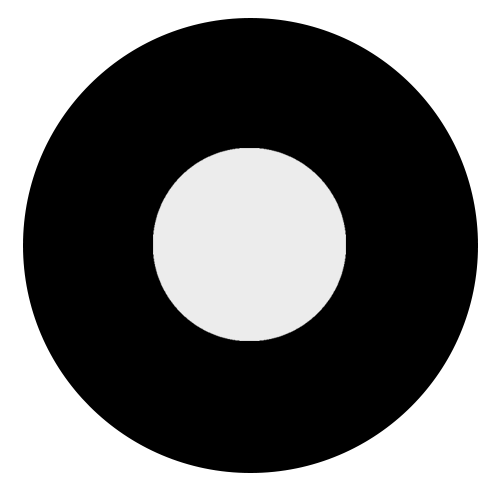
\includegraphics[width=0.12\textwidth]{Innen_klein.png}
		\hspace{10pt}
		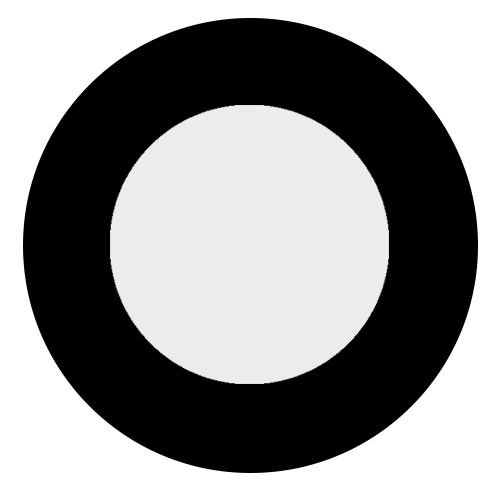
\includegraphics[width=0.12\textwidth]{Innen_mittel.png}
		\hspace{10pt}
		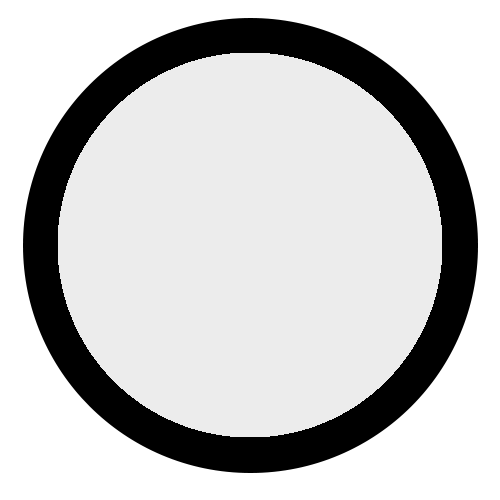
\includegraphics[width=0.12\textwidth]{Innen_gross.png}
		\hspace{10pt}
		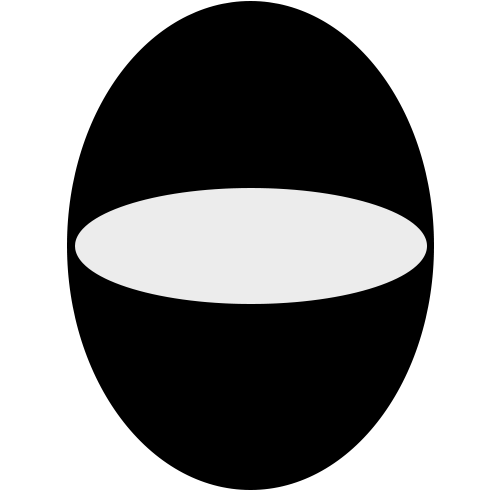
\includegraphics[width=0.12\textwidth]{Ellipsen.png}
	\end{center}
\end{figure}

\vspace{5pt}

Die entstandenen Bilder ben\"otigten zwischen 12 und 20 Iterationen, um die Stabilit\"at erkennbar zu machen.

\begin{figure}[h!]
	\frame{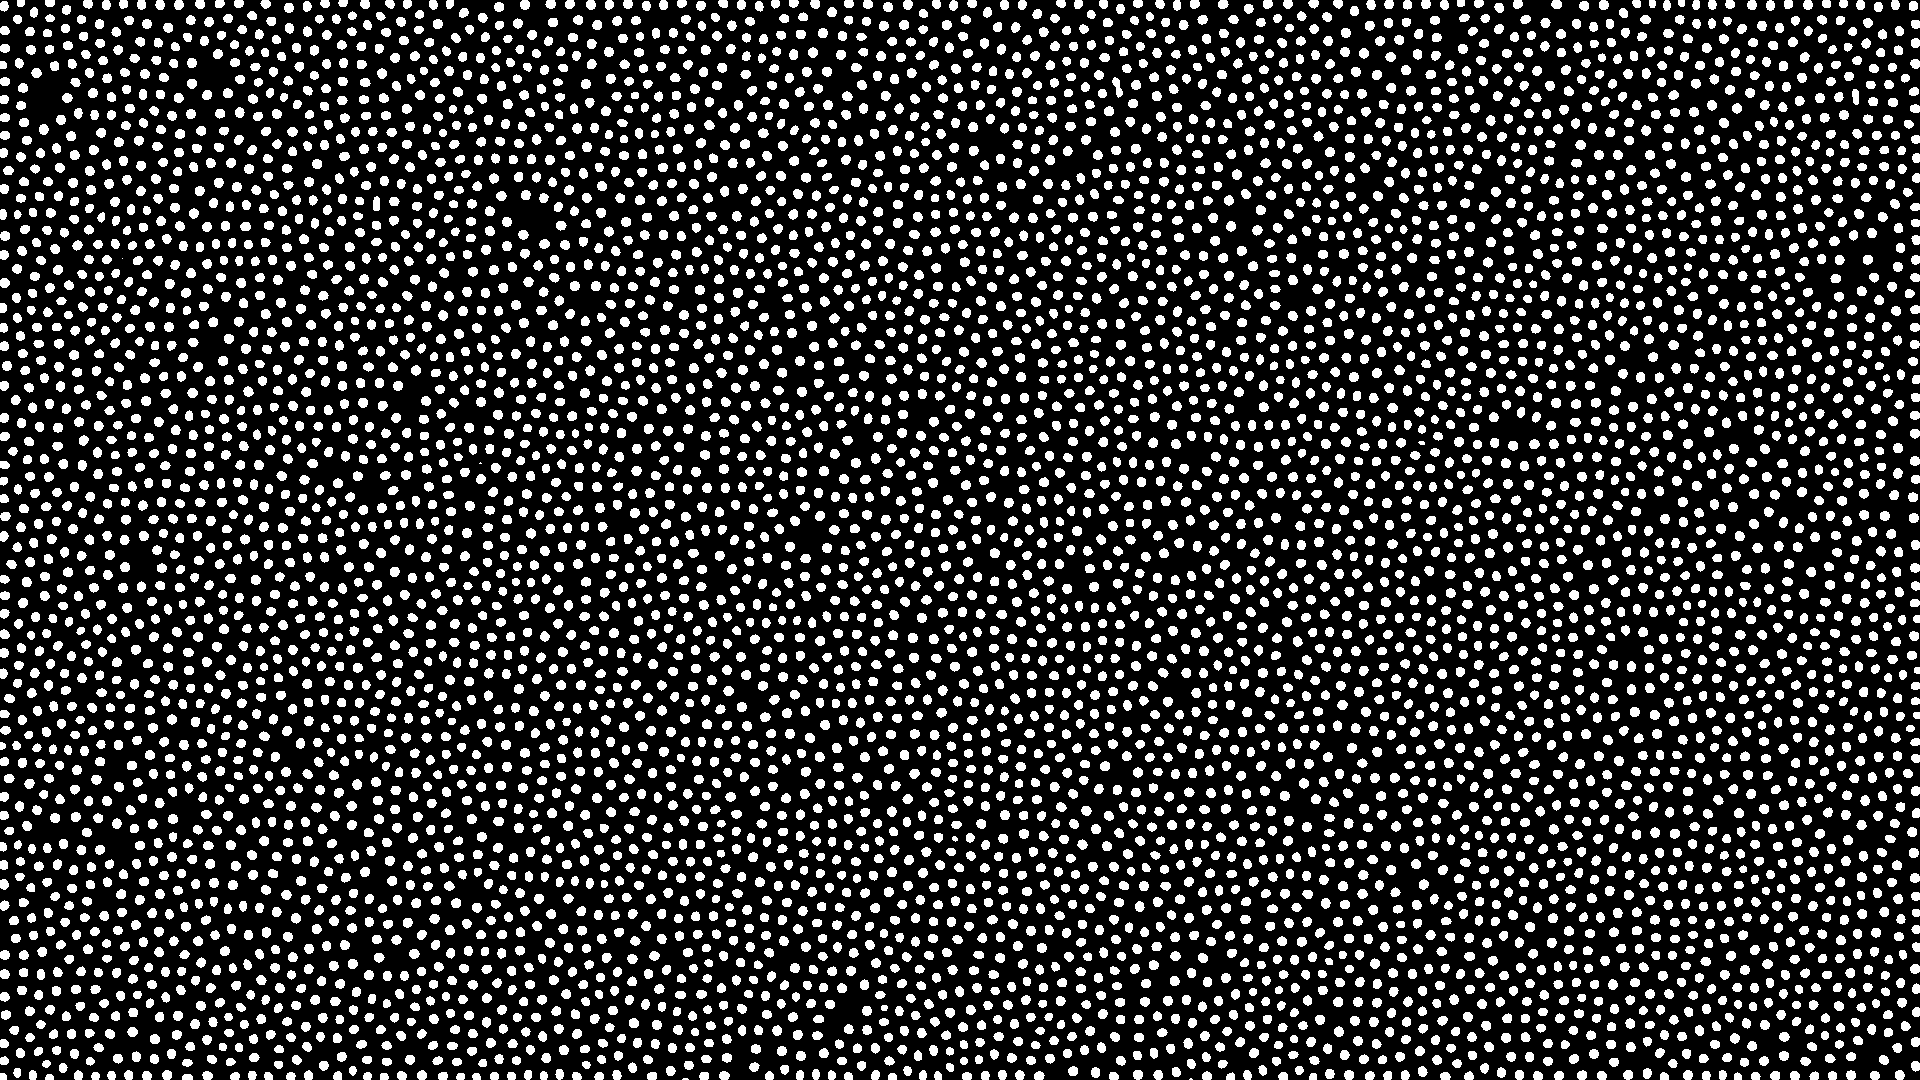
\includegraphics[width=\textwidth]{punkte.png}}
	\caption{Es entstehen Punkte, wenn der innere Radius 6, der \"au\ss ere Radius 11 und die zuf\"allige Chance einer Zelle zu Anfang gef\"arbt zu werden 1:20 betr\"agt.}
\end{figure}

\newpage

\begin{figure}[h!]
	\frame{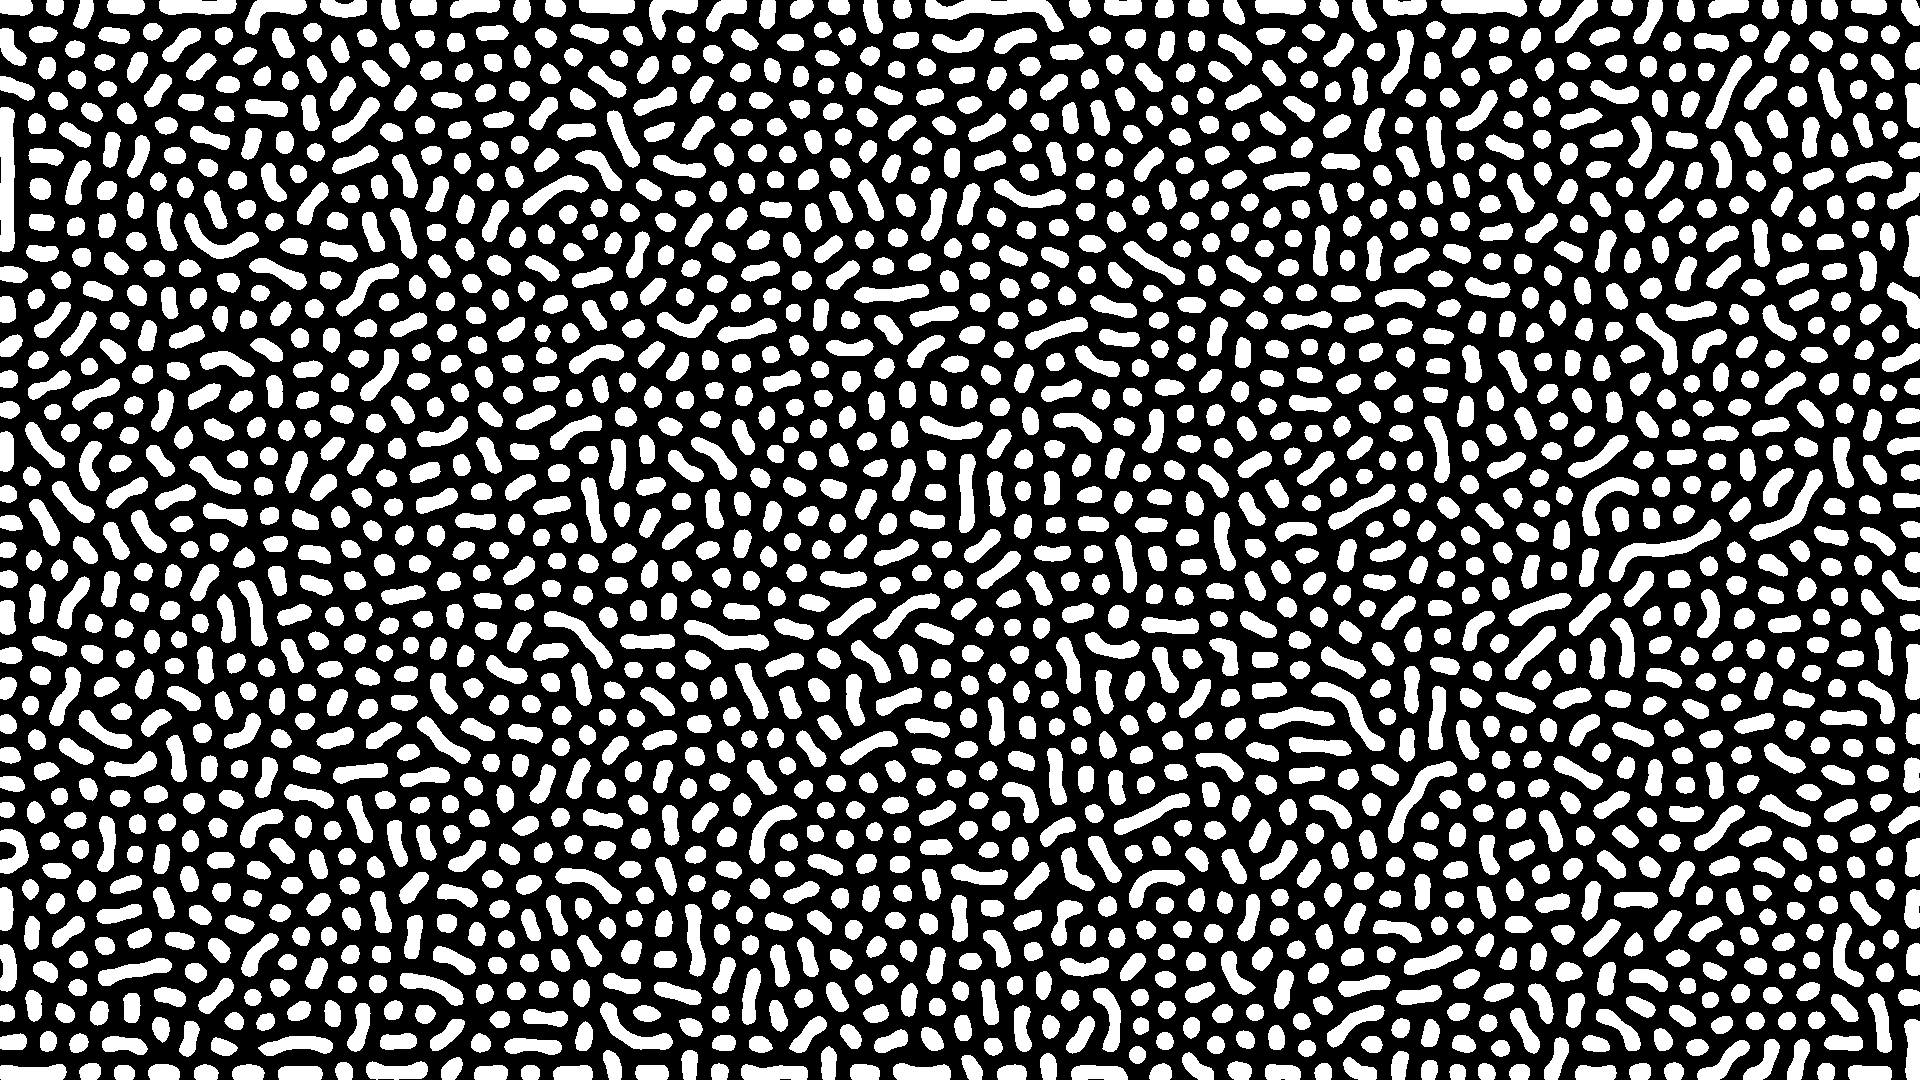
\includegraphics[width=\textwidth]{halb.png}}
	\caption{Es entstehen l\"angere zusammneh\"angende St\"ucke wie W\"urmer, wenn der innere Radius 12, der \"au\ss ere Radius 18 und die zuf\"allige Chance einer Zelle zu Anfang gef\"arbt zu werden 1:16 betr\"agt.}
\end{figure}

\begin{figure}[h!]
	\frame{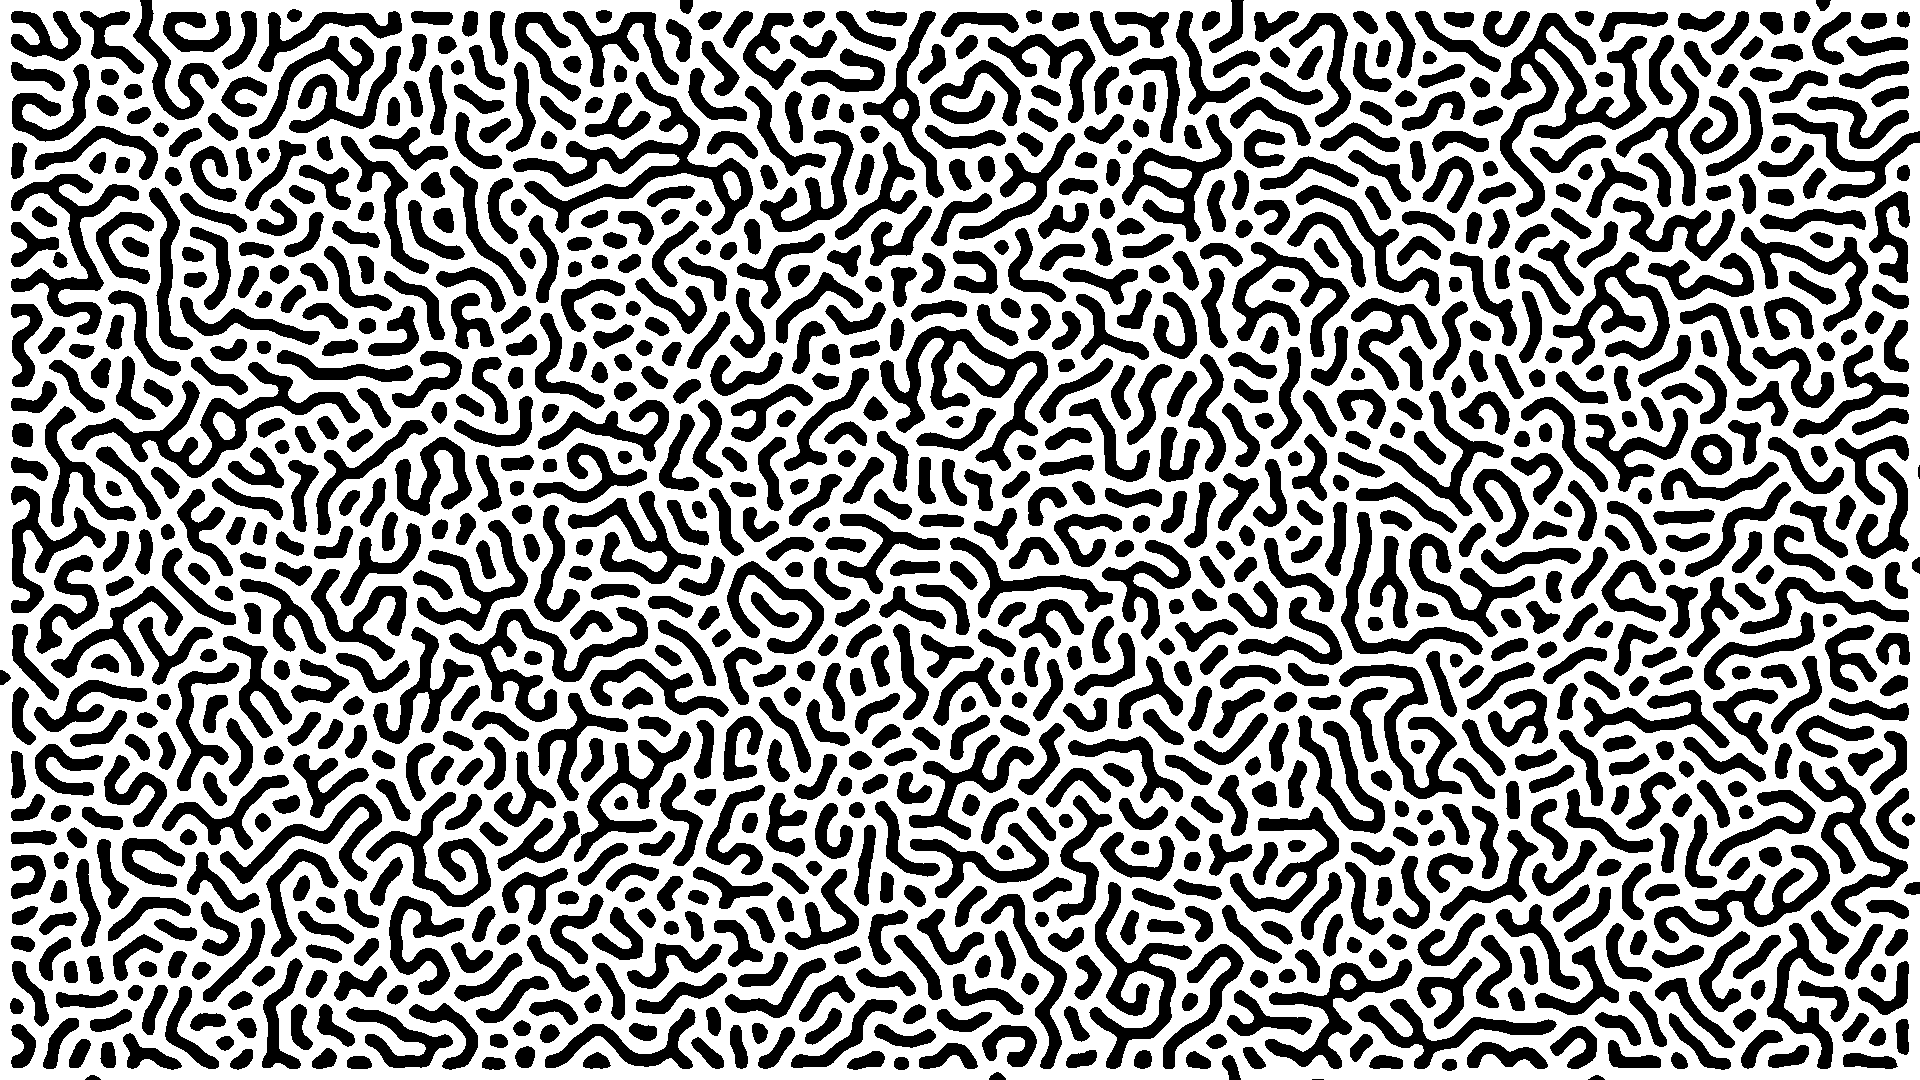
\includegraphics[width=\textwidth]{labyrinth.png}}
	\caption{Es entsteht eine Art Labyrinth, wenn der innere Radius 10, der \"au\ss ere Radius 14  und die zuf\"allige Chance einer Zelle zu Anfang gef\"arbt zu werden 1:12 betr\"agt.}
\end{figure}

\newpage

\begin{figure}[h!]
	\frame{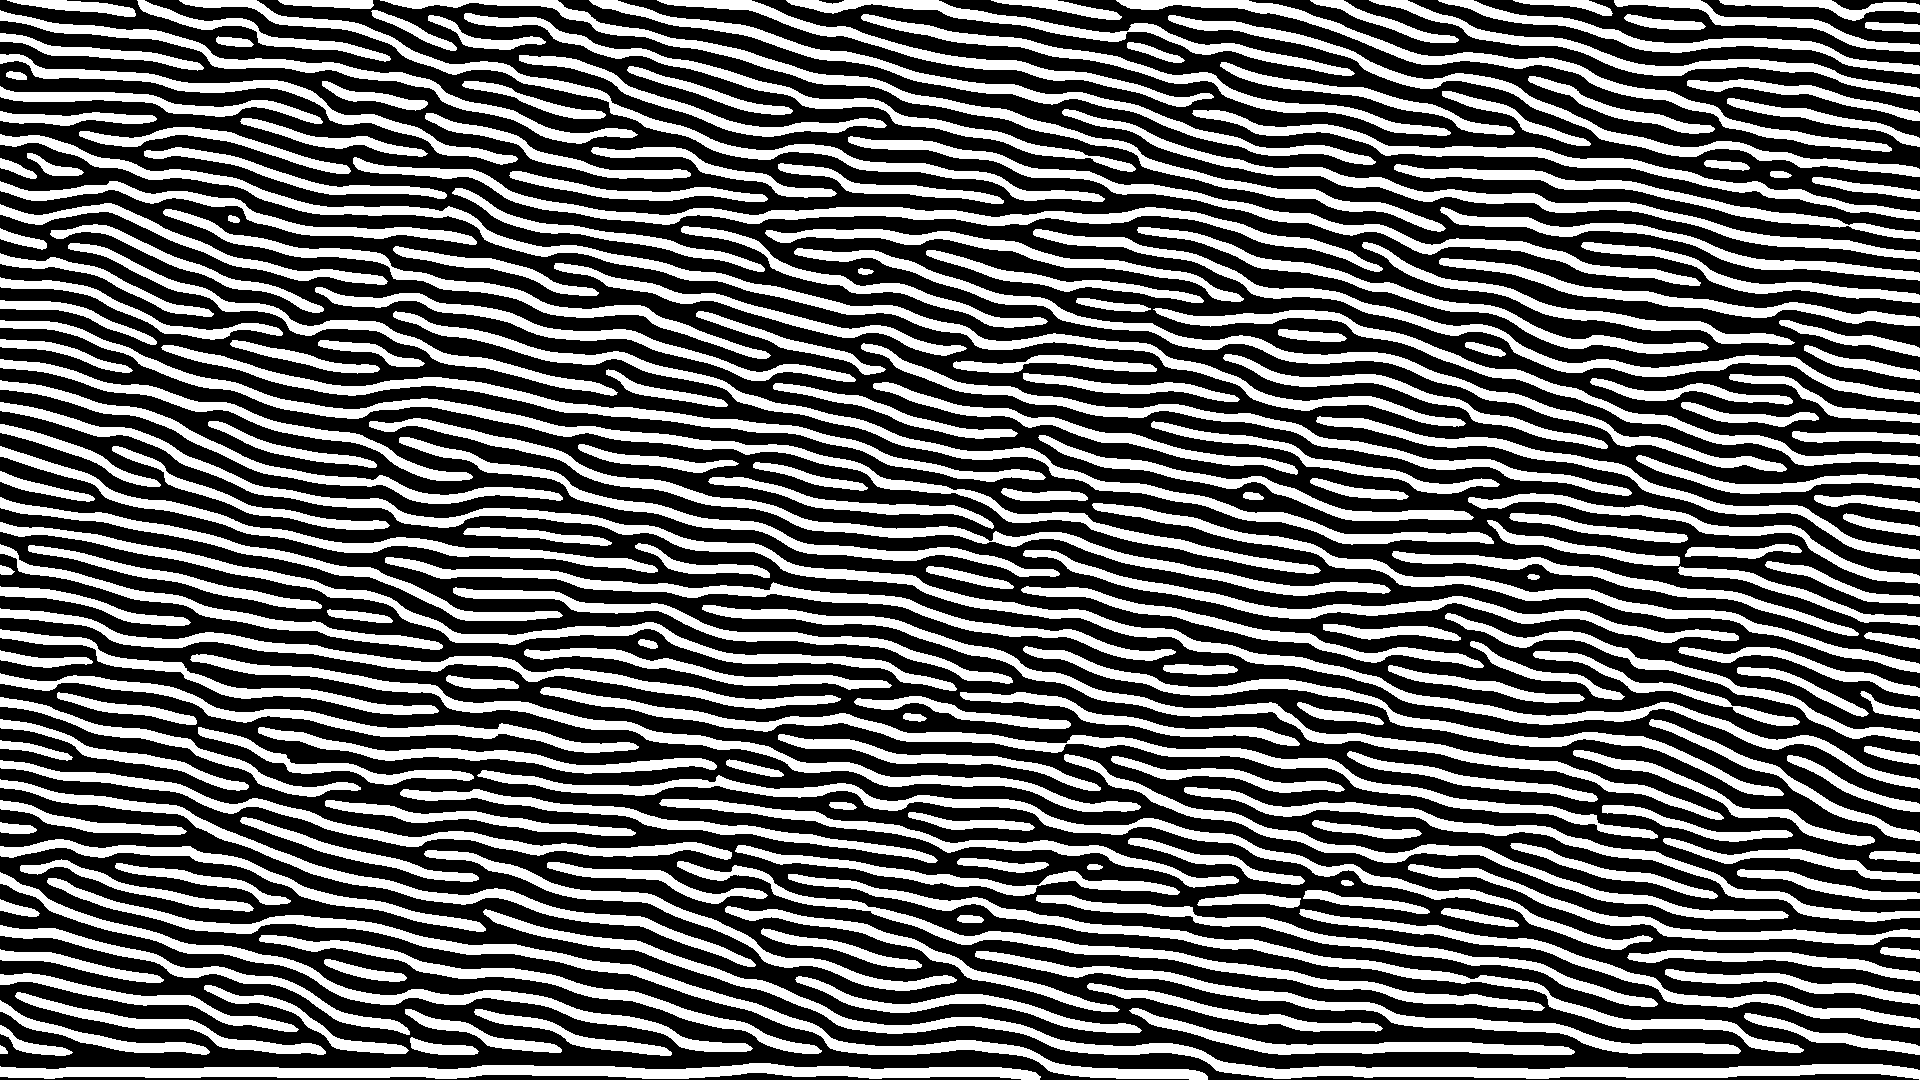
\includegraphics[width=\textwidth]{zebra.png}}
	\caption{Es entstehen Zebrastreifen, wenn die Ausma\ss e der Ellipsen 4 x 8 und 8 x 14 und die zuf\"allige Chance einer Zelle zu Anfang gef\"arbt zu werden 1:15 betragen.}
\end{figure}


\section{Benutzung und Features}

\subsection{Generierung neuer Patterns}
M\"ochte man ein neues Pattern generieren, muss man die Datei "UI.py" \"offnen, welche Abfragen in der Konsole stellt und anhand der Eingaben dann neue Patterns erstellt. Die dabei entstehenden Bilder werden in einem Unterordner namens "Generierte Bilder" gespeichert. Alle Iterationen eines Patterns werden in einem gemeinsamen Ordner gesammelt und durch die Informationen der Eingaben benannt. 

Das bedeutet, dass ein Ordner mit dem Namen "1920 x 1080 Modus 2 Chance 16 Ri 12 Ra 18" ein Bild mit der Aufl\"osung 1920 x 1080 Pixel ist, das im Modus 2 generiert wurde. Der Modus 2 steht dabei f\"ur einen Kreis und Ri und Ra stehen dabei jeweils f\"ur Innen- und Au\ss enradius; beide Werte sind in Pixeln angegeben. Desweiteren kann man an der Benennung erkennen, dass bei der Initiierung des Grids eine Wahrscheinlichkeit von 1 zu 16 bestand, dass eine Zelle ein Aktivator war. Die Bilder werden dann weiterhin mit dem Iterationsschritt benannt, sodass man diese leicht ordnen kann.

\subsection{Fortsetzung einer Berechnung}
Ein erg\"anzendes Feature ist die M\"oglichkeit vorhandene Bilder zu betrachten und anhand der Farben die Berechnungen fortzusetzen. Das erm\"oglicht sowohl die M\"oglichkeit Generierungen zu unterbrechen und  zu einem sp\"ateren Zeitpunkt fortzufahren, ein Bild (beispielsweise in Paint) zu erstellen und dieses dann als Grundlage f\"ur den Algorithmus zu nehmen oder aber wechselnde Zonen und Radien auf das gleiche Bild anzuwenden.

\subsection{Farbtausch}
Zu guter Letzt gibt das kurze Skript "ColourSwapping.py" die M\"oglichkeit, Farben in einem zweifarbigen Bild auszutauschen. Dadurch kann man tier\"ahnliche Farben in die Pattern-Generierung bringen. Dies hat eher einen veranschaulichenden Hintergrund als einen rein wissenschaftlichen. \\


\begin{figure}[h]
	\begin{center}
		\frame{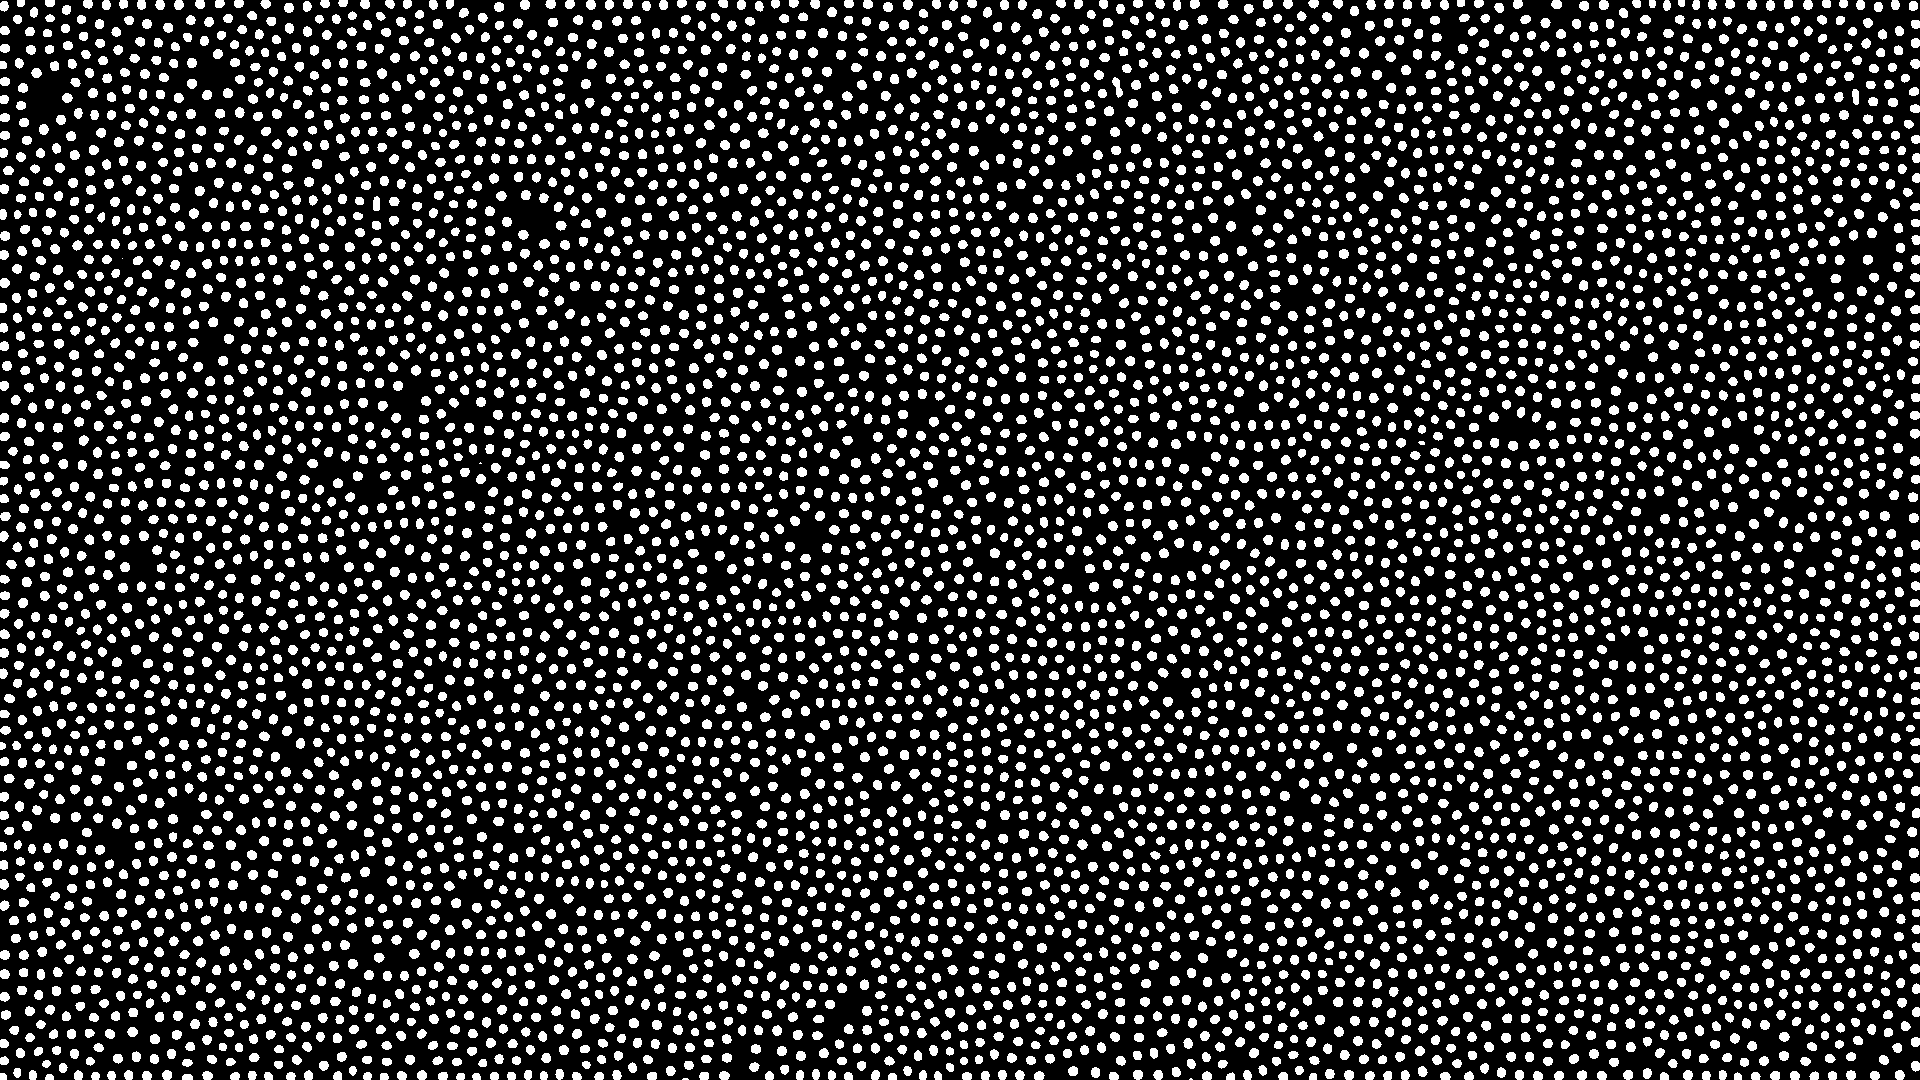
\includegraphics[trim=780 350 780 350, clip,width=0.22\textwidth]{punkte.png}}
		\hspace{50pt}
		\frame{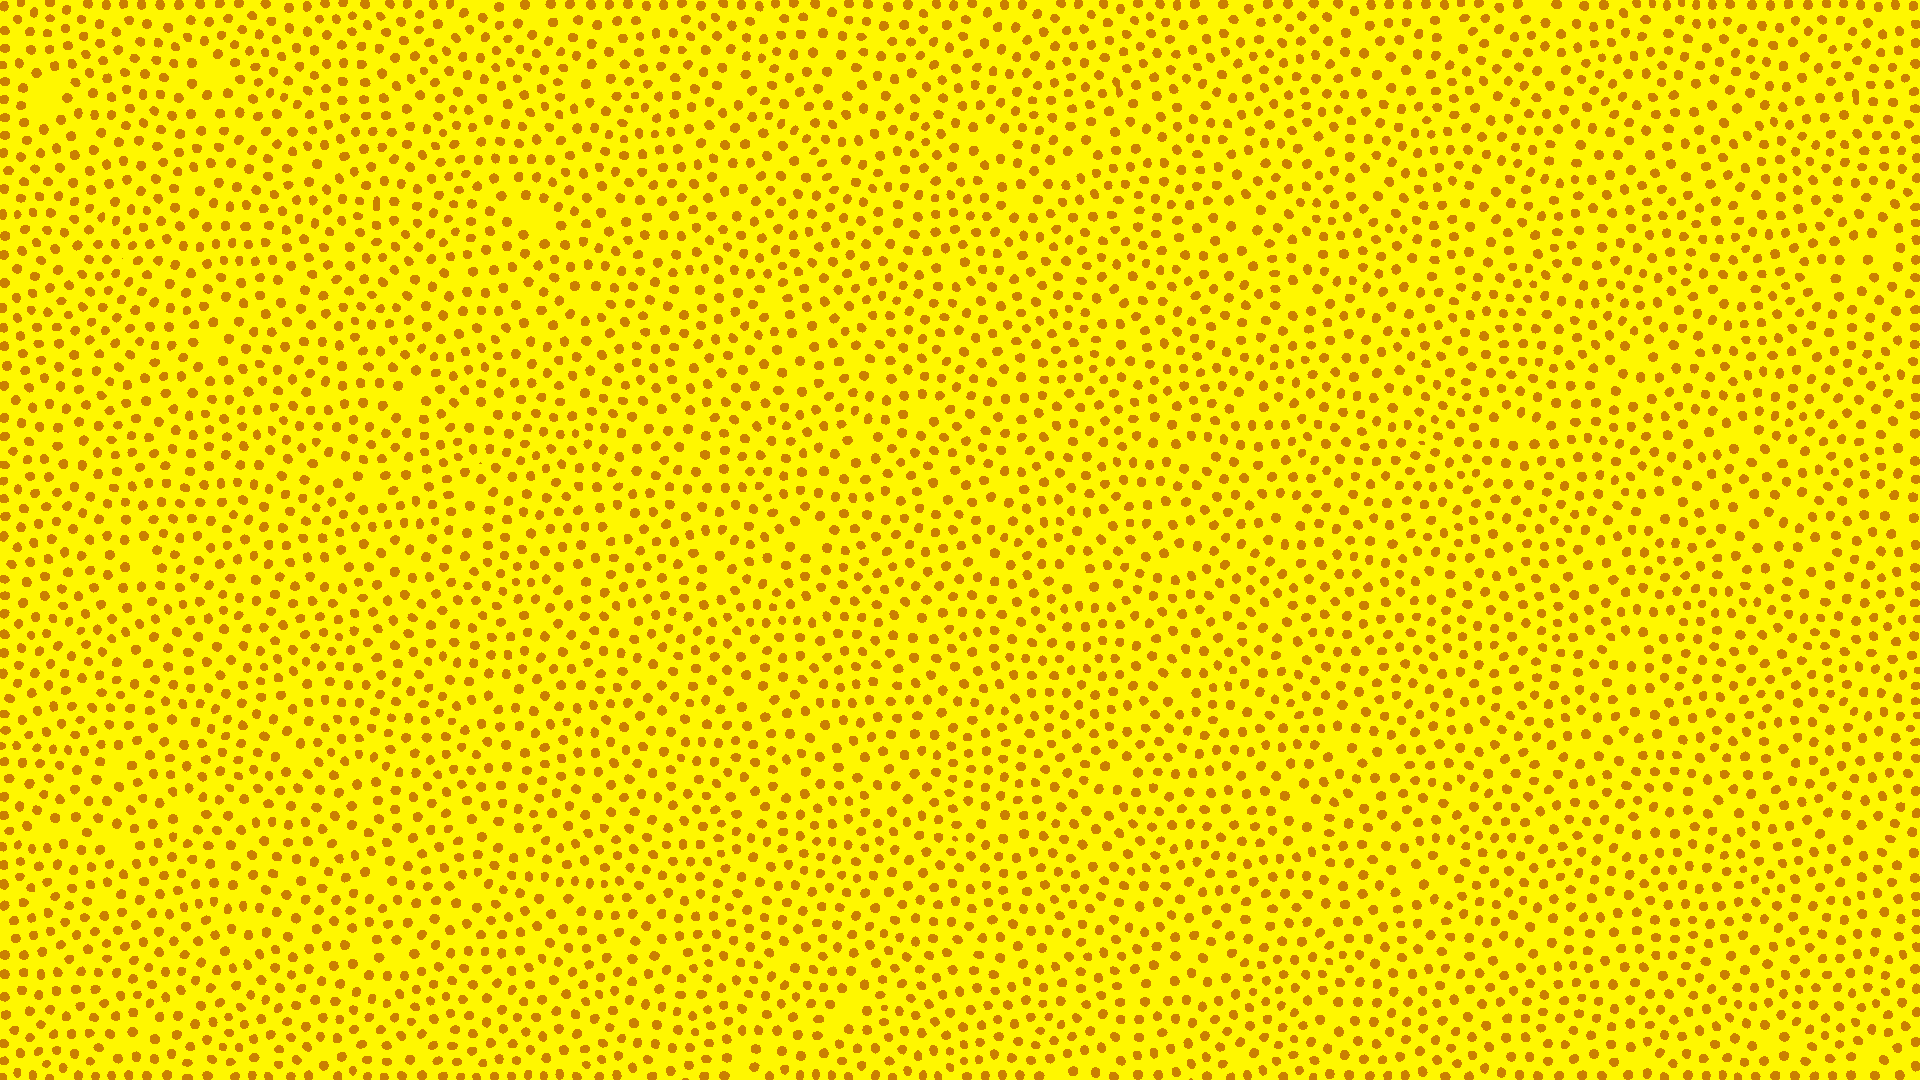
\includegraphics[trim=780 350 780 350, clip,width=0.22\textwidth]{leo.png}}
	\end{center}
\end{figure}


Zum Testen der Hintergrundmethoden kann man noch die Datei "CellMatrix.py" direkt in der Konsole \"offnen. Genaueres steht dazu in den Kommentaren ab Zeile 530.

\section{M\"ogliche Verbesserungen \& Erg\"anzungen}

\subsection{Andere Struktur}
Eine m\"ogliche Optimierung in der Struktur w\"are die Verwendung eines h\"oherdimensionalen Arrays, das dann die Nutzung der Unterklasse einer Zelle obsolet gemacht h\"atte. Wahrscheinlich handelt es sich dann um ein dreidimensionales Array, in denen dann die dritte Dimension zur Speicherung der Werte genommen worden w\"aren anstatt des Zellen-Objektes.
Dies h\"atte den weiteren Vorteil, dass pro Zelle zwei Integer weniger ben\"otigt werden, da man der Zelle nicht mehr explizit sagen muss, wo sie sich befindet.
Jedoch kam es als erstes zu der Entwicklung mit Zellen und danach erst wurden die Numpy-Arrays verwendet. Dies allein f\"uhrte schon zu einer deutlichen Verringerung der Berechnungszeit, jedoch h\"atte man f\"ur mehr Umstrukturierung viele der Funktionen neu modellieren m\"ussen und man h\"atte weniger Zeit zum Bilder erstellen gehabt. Da nicht bekannt war, in wie weit sich diese Umstellung zeitlich gelohnt h\"atte, konnte dieses Risiko nicht eingegangen werden und es wurde der sichere Weg bevorzugt, sodass wir zum Pr\"asentationstermin fertige Bilder pr\"asentieren konnten.

\subsection{Multithreading}
Der Gedanke zum Verwenden von Multithreading kam bereits relativ fr\"uh und wurde auch ein wenig getestet. Das Problem hierbei liegt allerdings in der Verwendung von Python und der Overhead, der beim Threading durch das Verschieben der Ergebnisse im Speicher generiert wird. 
Allerdings liegt dies auch daran, dass im ersten Versuch die Granulierung zum Erstellen der Threads zu klein gew\"ahlt wurde. So wurde mit jeder Zelle ein Thread generiert, welches bei gr\"o\ss eren Bildern nat\"urlich problematisch wird. Allerdings kam die Idee zur gr\"oberen Granulierung erst zu sp\"at w\"ahrend des Projektes auf. Das hatte dann zur Folge, dass die Umsetzung bis zur Pr\"asentation erst einmal gestrichen war, da man auch bei dieser Verbesserung nicht sicher sein konnte, ob es sich  tats\"achlich lohnen w\"urde, diese Zeit zu investieren.
Eine m\"ogliche Verbesserung dieses Problems in der Zukunft  k\"onnte eine Aufteilung entsprechend der Kerne sein, sodass dynamisch vom Programm entschieden wird, in wie viele Teile das Grid zur Berechnung unterteilt wird. Erkennt das Programm einen Vierkernprozessor, so wird das Gitter geviertelt, beim Sechskern gesechstelt und so weiter. Das bringt allerdings nur etwas, wenn Python tats\"achlich gut mit mehreren Threads skaliert und man sich sicher sein kann, dass das entsprechende Betriebssystem diese Aufgaben auch gleichm\"a\ss ig auf die Kerne verteilt.

\subsection{Konvergenz}
Damit ist gemeint, dass die Pattern-Generierung solange laufen soll, bis es zu keiner weiteren Ver\"anderung gegen\"uber der vorherigen Iteration mehr kommt.
Dieses Feature w\"are sehr sinnvoll zu erg\"anzen, da jedoch die Renderzeiten der einzelnen Bilder teilweise mehr als eine Stunde in Anspruch nahmen, h\"atte dieses Feature allerdings nie genutzt werden k\"onnen. Deshalb wurde es ausgelassen und stattdessen die M\"oglichkeit hinzugef\"ugt, die Berechnung abzubrechen und zu einem sp\"ateren Zeitpunkt weiterf\"uhren zu k\"onnen.

\subsection{Modulo-Betrachtung}
Hiermit ist lediglich die Betrachtung des Grids als herumreichende Ebene gemeint, sodass die Zellen an einem Ende des Gitters auch die Zellen am anderen Ende des Gitters mit in Betracht ziehen.
Dieses Feature wurde allerdings auch aufgrund von Zeitknappheit nicht weiter bearbeitet.

\begin{thebibliography}{9}
	
	\bibitem{greenfield2016}
	Greenfield, G. A. (2016). Turing-like Patterns from Cellular Automata. Proceedings of Bridges 2016, 151–158. 
	Abgerufen online unter http://archive.bridgesmathart.org/2016/bridges2016-151.html
	
	\bibitem{turing1952} 
	Turing, A. M. (1952). The chemical basis of morphogenesis. Philosophical Transactions of the Royal Society of London B: Biological Sciences, 237(641), 37-72.
	
	\bibitem{young1984}
		Young, D. A. (1984). A local activator-inhibitor model of vertebrate skin patterns. Mathematical Biosciences, 72(1), 51-58.
	
\end{thebibliography}

\end{document}
